\subsection*{Figure S1 -- structures fragment\'ees (avant / apr\`es)}
Pour chaque candidat fragment\'e (Tableau~S1)~: \`a gauche la g\'eom\'etrie initiale telle que produite par le criblage GFN2-xTB, \`a droite le r\'esultat de l'optimisation DFT WB97X-D4. La l\'egende sous chaque paire pr\'ecise si la g\'eom\'etrie initiale \'etait d\'ej\`a fragment\'ee \`a xTB (artefact du criblage en amont) ou encore intacte (fragmentation survenue pendant l'optimisation DFT elle-m\^eme).
\begin{figure}[H]
\centering
\begin{minipage}{0.46\textwidth}
\centering
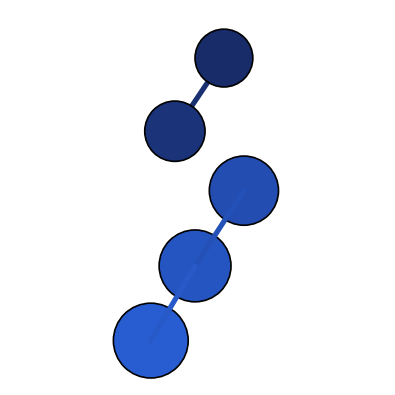
\includegraphics[width=0.8\linewidth]{figs/fragmented/N5_anion_anion_002_initial.png}\\[2pt]
{\small initiale (xTB, d\'ej\`a fragment\'ee, 2$+$3)}
\end{minipage}\hfill
\begin{minipage}{0.46\textwidth}
\centering
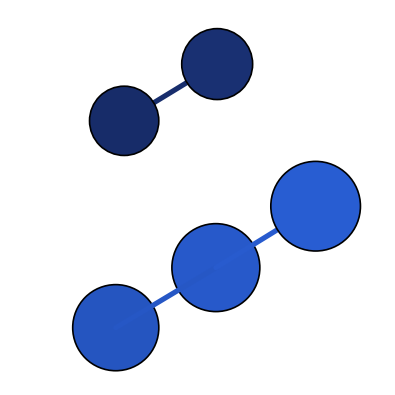
\includegraphics[width=0.8\linewidth]{figs/fragmented/N5_anion_anion_002_final.png}\\[2pt]
{\small DFT (fragment\'ee, 2$+$3)}
\end{minipage}
\end{figure}
\centerline{\small \texttt{N5\_anion\_anion\_002} -- fragments de taille 2$+$3}
\vspace{8pt}
\begin{figure}[H]
\centering
\begin{minipage}{0.46\textwidth}
\centering
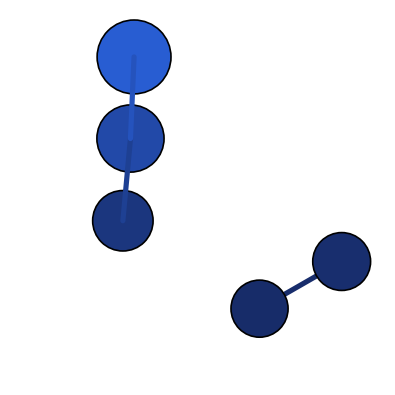
\includegraphics[width=0.8\linewidth]{figs/fragmented/N5_anion_anion_003_initial.png}\\[2pt]
{\small initiale (xTB, d\'ej\`a fragment\'ee, 2$+$3)}
\end{minipage}\hfill
\begin{minipage}{0.46\textwidth}
\centering
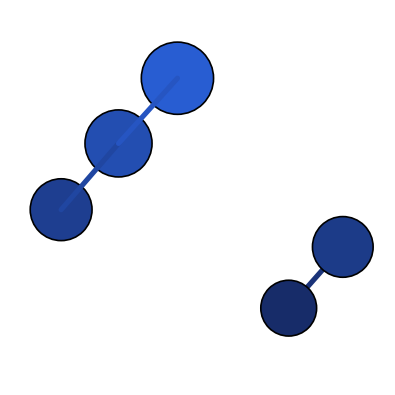
\includegraphics[width=0.8\linewidth]{figs/fragmented/N5_anion_anion_003_final.png}\\[2pt]
{\small DFT (fragment\'ee, 2$+$3)}
\end{minipage}
\end{figure}
\centerline{\small \texttt{N5\_anion\_anion\_003} -- fragments de taille 2$+$3}
\vspace{8pt}
\begin{figure}[H]
\centering
\begin{minipage}{0.46\textwidth}
\centering
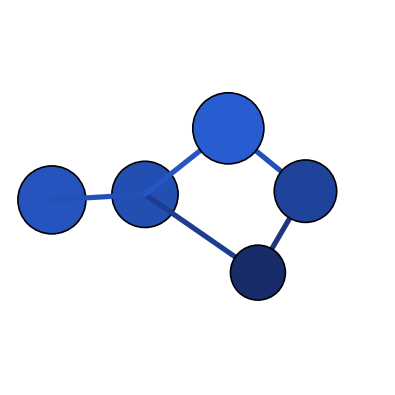
\includegraphics[width=0.8\linewidth]{figs/fragmented/N5_anion_anion_004_initial.png}\\[2pt]
{\small initiale (xTB, intacte, N$_5^{-}$)}
\end{minipage}\hfill
\begin{minipage}{0.46\textwidth}
\centering
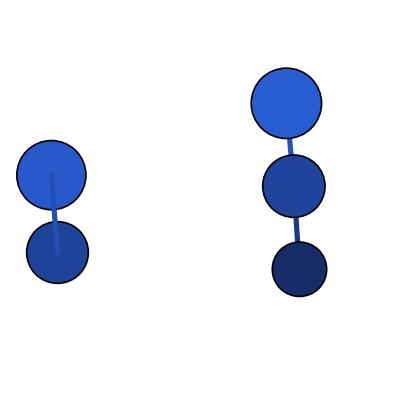
\includegraphics[width=0.8\linewidth]{figs/fragmented/N5_anion_anion_004_final.png}\\[2pt]
{\small DFT (fragment\'ee, 2$+$3)}
\end{minipage}
\end{figure}
\centerline{\small \texttt{N5\_anion\_anion\_004} -- fragments de taille 2$+$3}
\vspace{8pt}
\begin{figure}[H]
\centering
\begin{minipage}{0.46\textwidth}
\centering
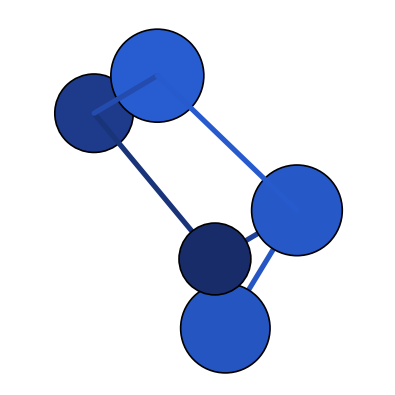
\includegraphics[width=0.8\linewidth]{figs/fragmented/N5_anion_anion_005_initial.png}\\[2pt]
{\small initiale (xTB, d\'ej\`a fragment\'ee, 2$+$3)}
\end{minipage}\hfill
\begin{minipage}{0.46\textwidth}
\centering
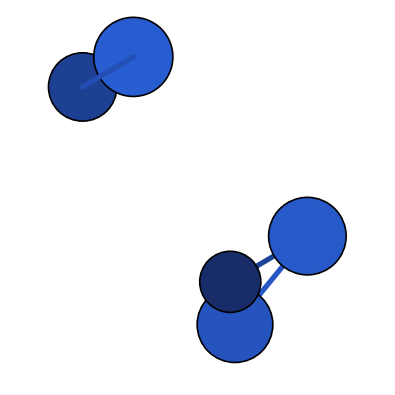
\includegraphics[width=0.8\linewidth]{figs/fragmented/N5_anion_anion_005_final.png}\\[2pt]
{\small DFT (fragment\'ee, 2$+$3)}
\end{minipage}
\end{figure}
\centerline{\small \texttt{N5\_anion\_anion\_005} -- fragments de taille 2$+$3}
\vspace{8pt}
\begin{figure}[H]
\centering
\begin{minipage}{0.46\textwidth}
\centering
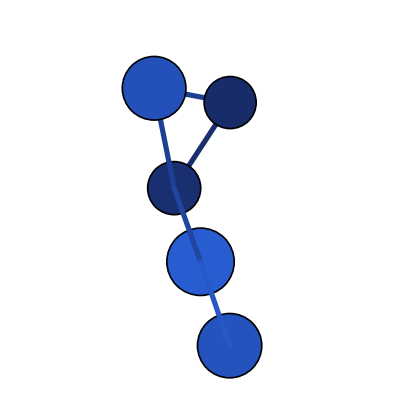
\includegraphics[width=0.8\linewidth]{figs/fragmented/N5_anion_anion_007_initial.png}\\[2pt]
{\small initiale (xTB, intacte, N$_5^{-}$)}
\end{minipage}\hfill
\begin{minipage}{0.46\textwidth}
\centering
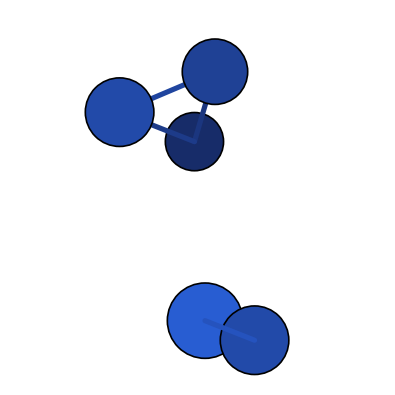
\includegraphics[width=0.8\linewidth]{figs/fragmented/N5_anion_anion_007_final.png}\\[2pt]
{\small DFT (fragment\'ee, 2$+$3)}
\end{minipage}
\end{figure}
\centerline{\small \texttt{N5\_anion\_anion\_007} -- fragments de taille 2$+$3}
\vspace{8pt}
\begin{figure}[H]
\centering
\begin{minipage}{0.46\textwidth}
\centering
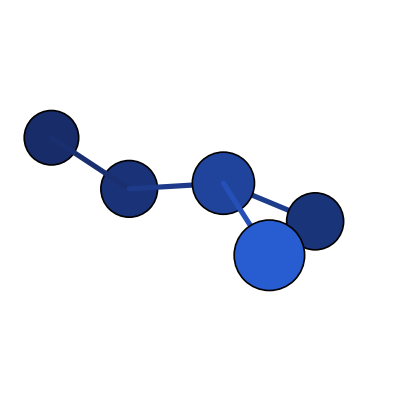
\includegraphics[width=0.8\linewidth]{figs/fragmented/N5_anion_anion_008_initial.png}\\[2pt]
{\small initiale (xTB, intacte, N$_5^{-}$)}
\end{minipage}\hfill
\begin{minipage}{0.46\textwidth}
\centering
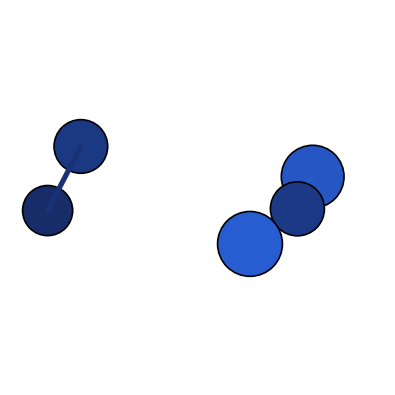
\includegraphics[width=0.8\linewidth]{figs/fragmented/N5_anion_anion_008_final.png}\\[2pt]
{\small DFT (fragment\'ee, 2$+$3)}
\end{minipage}
\end{figure}
\centerline{\small \texttt{N5\_anion\_anion\_008} -- fragments de taille 2$+$3}
\vspace{8pt}
\begin{figure}[H]
\centering
\begin{minipage}{0.46\textwidth}
\centering
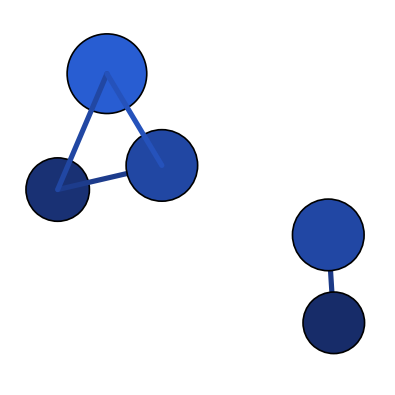
\includegraphics[width=0.8\linewidth]{figs/fragmented/N5_anion_anion_009_initial.png}\\[2pt]
{\small initiale (xTB, d\'ej\`a fragment\'ee, 2$+$3)}
\end{minipage}\hfill
\begin{minipage}{0.46\textwidth}
\centering
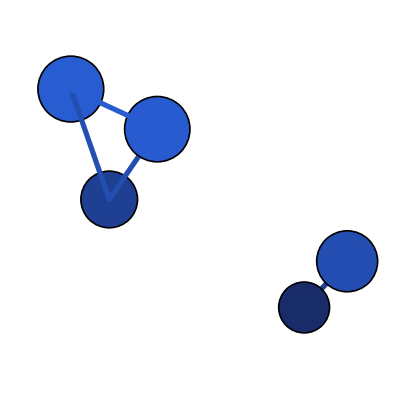
\includegraphics[width=0.8\linewidth]{figs/fragmented/N5_anion_anion_009_final.png}\\[2pt]
{\small DFT (fragment\'ee, 2$+$3)}
\end{minipage}
\end{figure}
\centerline{\small \texttt{N5\_anion\_anion\_009} -- fragments de taille 2$+$3}
\vspace{8pt}
\begin{figure}[H]
\centering
\begin{minipage}{0.46\textwidth}
\centering
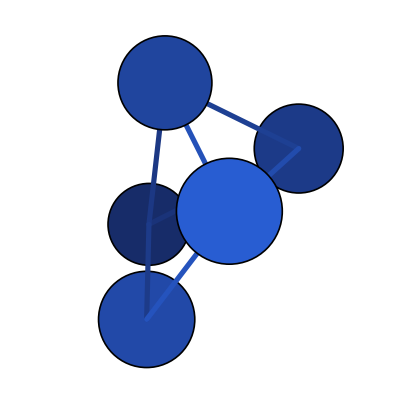
\includegraphics[width=0.8\linewidth]{figs/fragmented/N5_cation_cation_007_initial.png}\\[2pt]
{\small initiale (xTB, intacte, N$_5^{+}$)}
\end{minipage}\hfill
\begin{minipage}{0.46\textwidth}
\centering
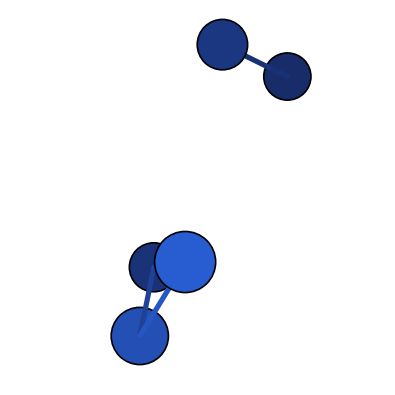
\includegraphics[width=0.8\linewidth]{figs/fragmented/N5_cation_cation_007_final.png}\\[2pt]
{\small DFT (fragment\'ee, 2$+$3)}
\end{minipage}
\end{figure}
\centerline{\small \texttt{N5\_cation\_cation\_007} -- fragments de taille 2$+$3}
\vspace{8pt}
\begin{figure}[H]
\centering
\begin{minipage}{0.46\textwidth}
\centering
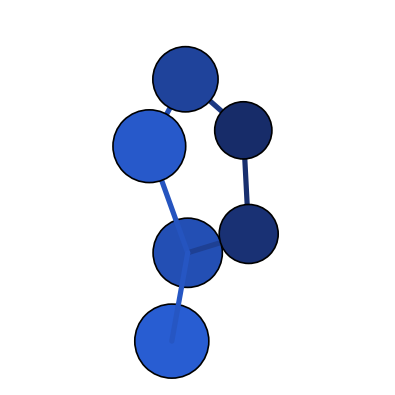
\includegraphics[width=0.8\linewidth]{figs/fragmented/N6_neutral_neutral_004_initial.png}\\[2pt]
{\small initiale (xTB, intacte, N$_6^{0}$)}
\end{minipage}\hfill
\begin{minipage}{0.46\textwidth}
\centering
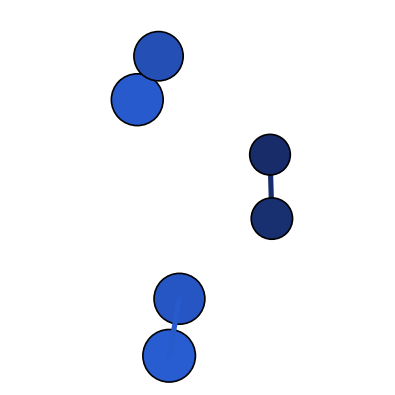
\includegraphics[width=0.8\linewidth]{figs/fragmented/N6_neutral_neutral_004_final.png}\\[2pt]
{\small DFT (fragment\'ee, 2$+$2$+$2)}
\end{minipage}
\end{figure}
\centerline{\small \texttt{N6\_neutral\_neutral\_004} -- fragments de taille 2$+$2$+$2}
\vspace{8pt}
\begin{figure}[H]
\centering
\begin{minipage}{0.46\textwidth}
\centering
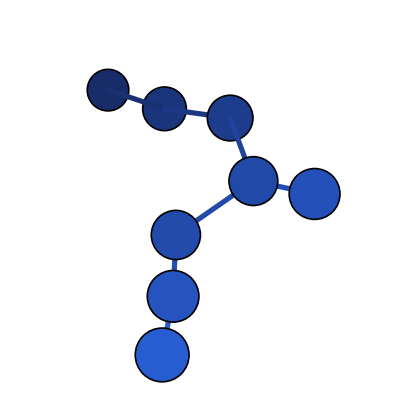
\includegraphics[width=0.8\linewidth]{figs/fragmented/N8_neutral_neutral_006_initial.png}\\[2pt]
{\small initiale (xTB, intacte, N$_8^{0}$)}
\end{minipage}\hfill
\begin{minipage}{0.46\textwidth}
\centering
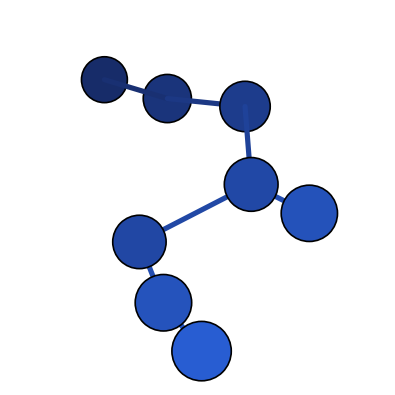
\includegraphics[width=0.8\linewidth]{figs/fragmented/N8_neutral_neutral_006_final.png}\\[2pt]
{\small DFT (fragment\'ee, 3$+$5)}
\end{minipage}
\end{figure}
\centerline{\small \texttt{N8\_neutral\_neutral\_006} -- fragments de taille 3$+$5}
\vspace{8pt}
\begin{figure}[H]
\centering
\begin{minipage}{0.46\textwidth}
\centering
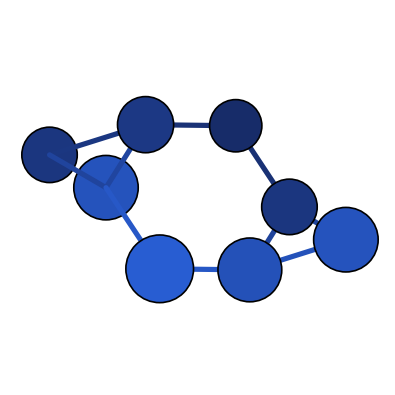
\includegraphics[width=0.8\linewidth]{figs/fragmented/N8_neutral_neutral_018_initial.png}\\[2pt]
{\small initiale (xTB, intacte, N$_8^{0}$)}
\end{minipage}\hfill
\begin{minipage}{0.46\textwidth}
\centering
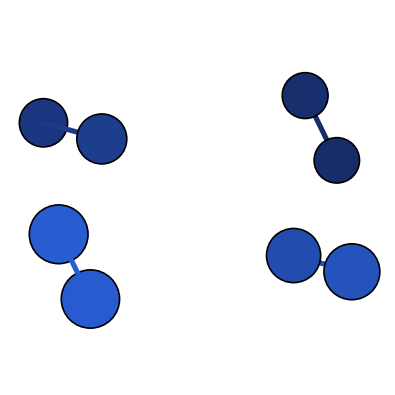
\includegraphics[width=0.8\linewidth]{figs/fragmented/N8_neutral_neutral_018_final.png}\\[2pt]
{\small DFT (fragment\'ee, 2$+$2$+$2$+$2)}
\end{minipage}
\end{figure}
\centerline{\small \texttt{N8\_neutral\_neutral\_018} -- fragments de taille 2$+$2$+$2$+$2}
\vspace{8pt}
\begin{figure}[H]
\centering
\begin{minipage}{0.46\textwidth}
\centering
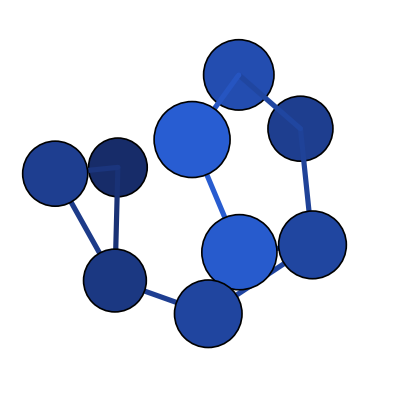
\includegraphics[width=0.8\linewidth]{figs/fragmented/N9_anion_anion_015_initial.png}\\[2pt]
{\small initiale (xTB, intacte, N$_9^{-}$)}
\end{minipage}\hfill
\begin{minipage}{0.46\textwidth}
\centering
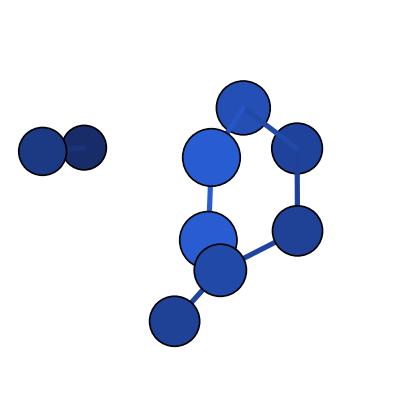
\includegraphics[width=0.8\linewidth]{figs/fragmented/N9_anion_anion_015_final.png}\\[2pt]
{\small DFT (fragment\'ee, 2$+$7)}
\end{minipage}
\end{figure}
\centerline{\small \texttt{N9\_anion\_anion\_015} -- fragments de taille 2$+$7}
\vspace{8pt}
\begin{figure}[H]
\centering
\begin{minipage}{0.46\textwidth}
\centering
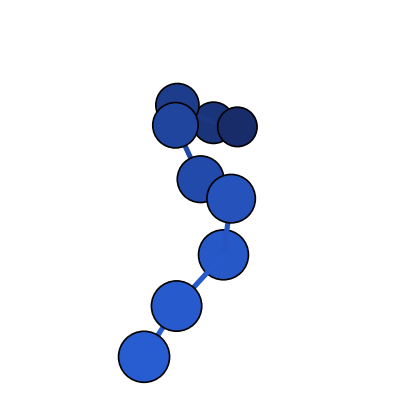
\includegraphics[width=0.8\linewidth]{figs/fragmented/N9_cation_cation_001_initial.png}\\[2pt]
{\small initiale (xTB, intacte, N$_9^{+}$)}
\end{minipage}\hfill
\begin{minipage}{0.46\textwidth}
\centering
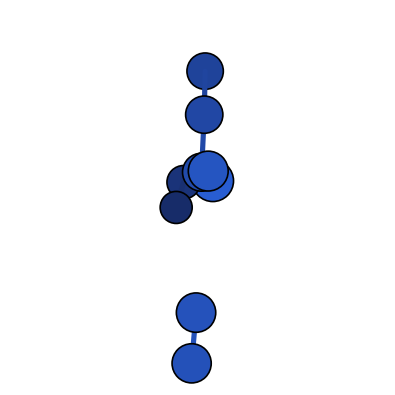
\includegraphics[width=0.8\linewidth]{figs/fragmented/N9_cation_cation_001_final.png}\\[2pt]
{\small DFT (fragment\'ee, 2$+$2$+$5)}
\end{minipage}
\end{figure}
\centerline{\small \texttt{N9\_cation\_cation\_001} -- fragments de taille 2$+$2$+$5}
\vspace{8pt}
\begin{figure}[H]
\centering
\begin{minipage}{0.46\textwidth}
\centering
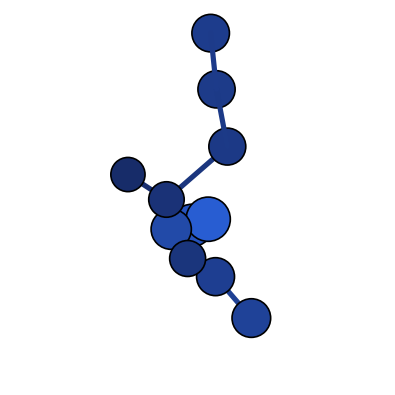
\includegraphics[width=0.8\linewidth]{figs/fragmented/N11_anion_anion_011_initial.png}\\[2pt]
{\small initiale (xTB, d\'ej\`a fragment\'ee, 3$+$3$+$5)}
\end{minipage}\hfill
\begin{minipage}{0.46\textwidth}
\centering
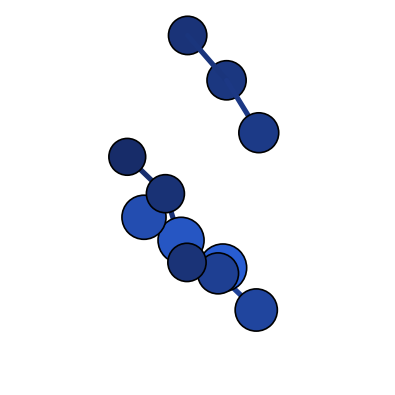
\includegraphics[width=0.8\linewidth]{figs/fragmented/N11_anion_anion_011_final.png}\\[2pt]
{\small DFT (fragment\'ee, 3$+$3$+$5)}
\end{minipage}
\end{figure}
\centerline{\small \texttt{N11\_anion\_anion\_011} -- fragments de taille 3$+$3$+$5}
\vspace{8pt}
\begin{figure}[H]
\centering
\begin{minipage}{0.46\textwidth}
\centering
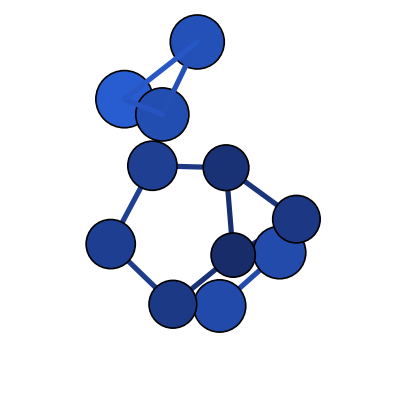
\includegraphics[width=0.8\linewidth]{figs/fragmented/N11_anion_anion_018_initial.png}\\[2pt]
{\small initiale (xTB, intacte, N$_11^{-}$)}
\end{minipage}\hfill
\begin{minipage}{0.46\textwidth}
\centering
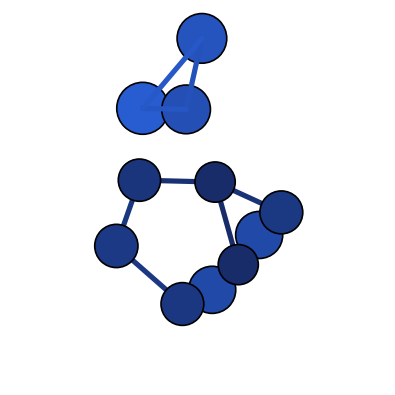
\includegraphics[width=0.8\linewidth]{figs/fragmented/N11_anion_anion_018_final.png}\\[2pt]
{\small DFT (fragment\'ee, 3$+$8)}
\end{minipage}
\end{figure}
\centerline{\small \texttt{N11\_anion\_anion\_018} -- fragments de taille 3$+$8}
\vspace{8pt}
\begin{figure}[H]
\centering
\begin{minipage}{0.46\textwidth}
\centering
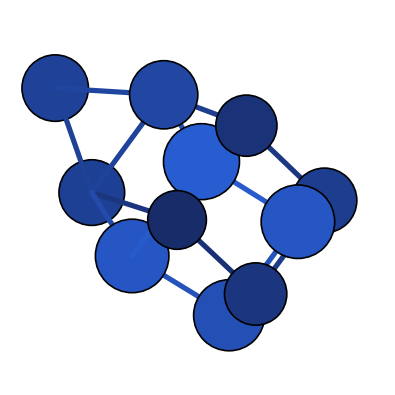
\includegraphics[width=0.8\linewidth]{figs/fragmented/N11_cation_cation_009_initial.png}\\[2pt]
{\small initiale (xTB, intacte, N$_11^{+}$)}
\end{minipage}\hfill
\begin{minipage}{0.46\textwidth}
\centering
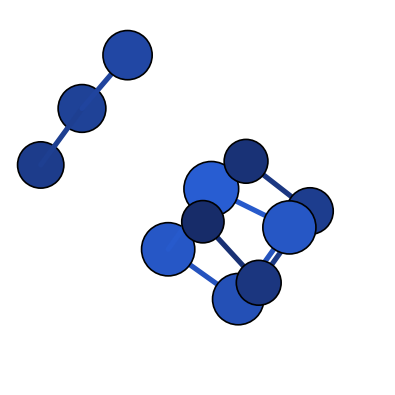
\includegraphics[width=0.8\linewidth]{figs/fragmented/N11_cation_cation_009_final.png}\\[2pt]
{\small DFT (fragment\'ee, 3$+$8)}
\end{minipage}
\end{figure}
\centerline{\small \texttt{N11\_cation\_cation\_009} -- fragments de taille 3$+$8}
\vspace{8pt}
\begin{figure}[H]
\centering
\begin{minipage}{0.46\textwidth}
\centering
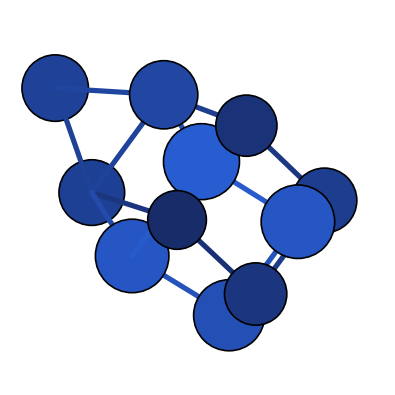
\includegraphics[width=0.8\linewidth]{figs/fragmented/N11_cation_cation_010_initial.png}\\[2pt]
{\small initiale (xTB, intacte, N$_11^{+}$)}
\end{minipage}\hfill
\begin{minipage}{0.46\textwidth}
\centering
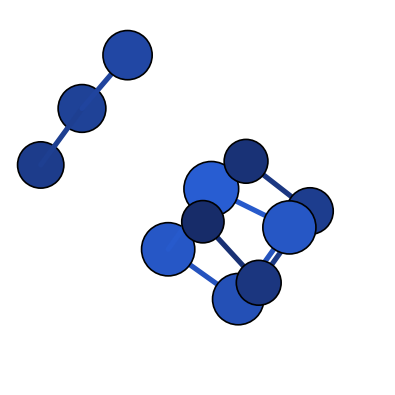
\includegraphics[width=0.8\linewidth]{figs/fragmented/N11_cation_cation_010_final.png}\\[2pt]
{\small DFT (fragment\'ee, 3$+$8)}
\end{minipage}
\end{figure}
\centerline{\small \texttt{N11\_cation\_cation\_010} -- fragments de taille 3$+$8}
\vspace{8pt}
\begin{figure}[H]
\centering
\begin{minipage}{0.46\textwidth}
\centering
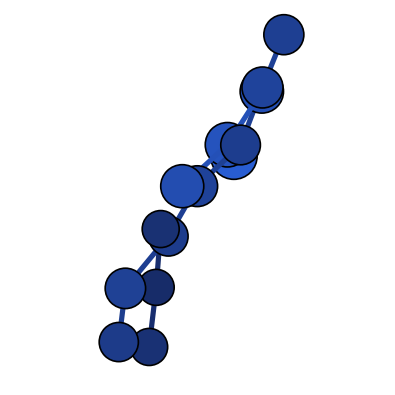
\includegraphics[width=0.8\linewidth]{figs/fragmented/N14_neutral_neutral_004_initial.png}\\[2pt]
{\small initiale (xTB, intacte, N$_14^{0}$)}
\end{minipage}\hfill
\begin{minipage}{0.46\textwidth}
\centering
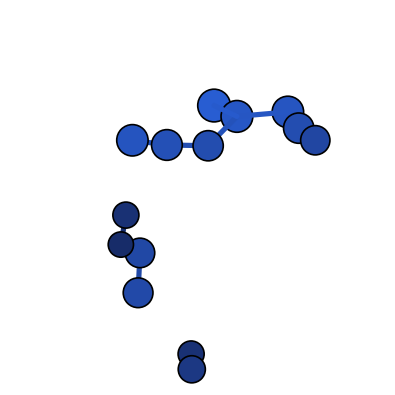
\includegraphics[width=0.8\linewidth]{figs/fragmented/N14_neutral_neutral_004_final.png}\\[2pt]
{\small DFT (fragment\'ee, 2$+$2$+$2$+$3$+$5)}
\end{minipage}
\end{figure}
\centerline{\small \texttt{N14\_neutral\_neutral\_004} -- fragments de taille 2$+$2$+$2$+$3$+$5}
\vspace{8pt}
\bigskip\noindent\textit{L\'egende g\'en\'erale, Figure~S1~:} sph\`eres bleues reli\'ees par des b\^atonnets = atomes N et liaisons N--N (mod\`ele boules-b\^atonnets, rendu depuis les coordonn\'ees cart\'esiennes .xyz) ; paires group\'ees par candidat, g\'eom\'etrie initiale GFN2-xTB \`a gauche et g\'eom\'etrie finale DFT WB97X-D4 \`a droite pour chacun des 18 candidats fragment\'es dont le calcul DFT est termin\'e (sur les 24 recens\'es au Tableau~S1 ; les autres n'ont pas encore de g\'eom\'etrie DFT \`a montrer).